\documentclass[10pt]{article}
\input preamble.tex
\sisetup{round-mode=places,round-precision=3}

\pagestyle{fancy}
\fancyhf{}
\lhead{CADIS Simulation Results}
\chead{12/11/2016}
\rhead{Caroline Hughes}
\renewcommand{\headrulewidth}{0pt}

\begin{document}

\section*{Sample Plots}

\begin{figure}[!h]
\centering
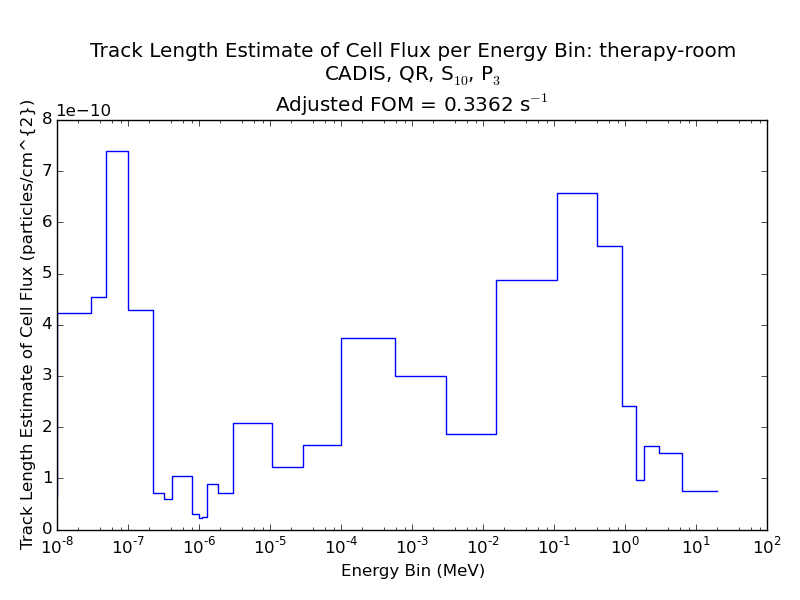
\includegraphics[width = 0.75\textwidth]{plot/tally-therapy-room_qr10-3.png}
\caption{Plot of track length estimate of cell flux per energy bin}
\end{figure}

\begin{figure}[!h]
\centering
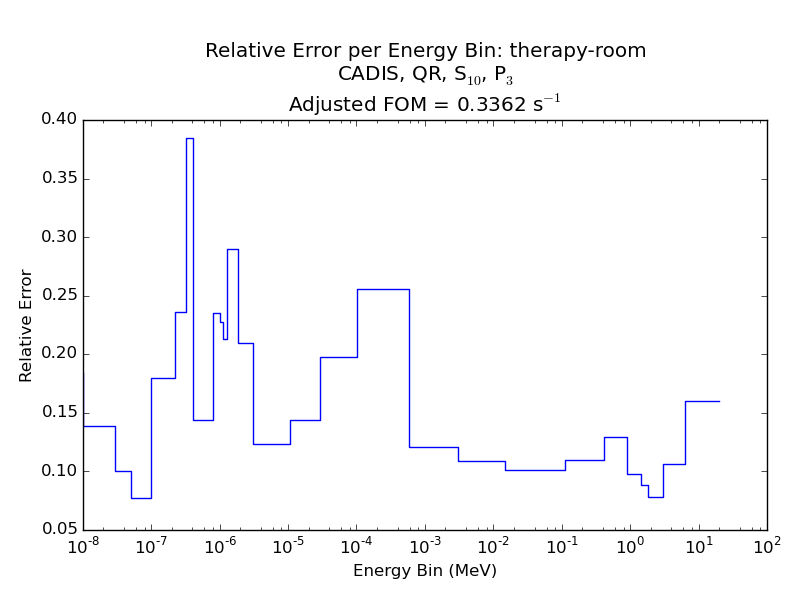
\includegraphics[width = 0.75\textwidth]{plot/sigma-therapy-room_qr10-3.png}
\caption{Plot of relative error per energy bin}
\end{figure}

\newpage 

\begin{figure}[!h]
\centering
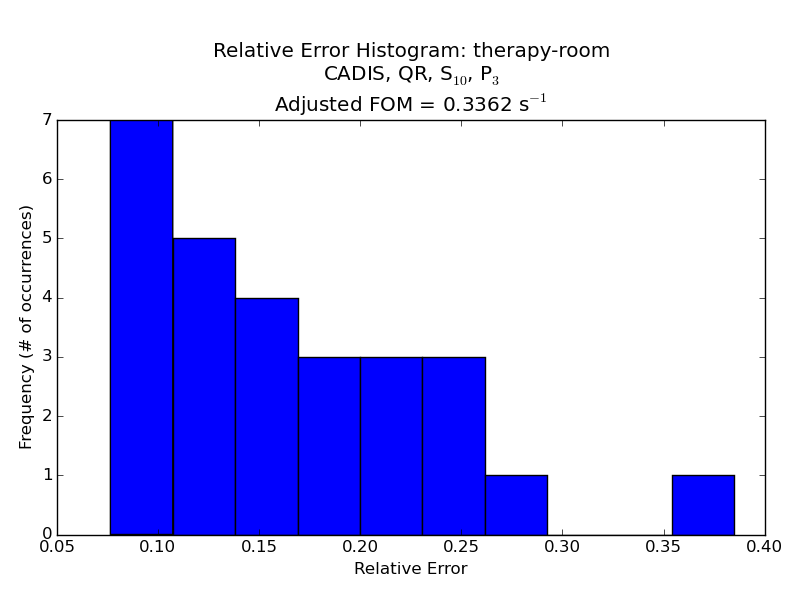
\includegraphics[width = 0.75\textwidth]{plot/hist-therapy-room_qr10-3.png}
\caption{Histogram of relative error distribution}
\end{figure}


I generated these three plots for each test case. They can be found for every test in

\texttt{/global/scratch/co$\_$nuclear/NE255project/MCNP/plots/cadis/}.

\newpage
\section*{Tables}

%%%%%%%%%%%%%%%%%%%%%%%%%%%%%%%%%%%%%%%%%%%%%%%%%%%%
%   BEAM
%%%%%%%%%%%%%%%%%%%%%%%%%%%%%%%%%%%%%%%%%%%%%%%%%%%%
\begin{table}[!h]
\centering
\caption{Beam}
\csvreader[head to column names,
    tabular = cSScSSSSSS,
    table head = \toprule
        &&&& {Max.}
        & \multicolumn{2}{c}{Run Time (\si{\second})}
        & \multicolumn{2}{c}{Figure of Merit (\si{\second^{-1}})}
        \\
          Quadrature
        & {$S_N$}
        & {$P_N$}
        & {Method}
        & {Rel. Err.}
        & {Denovo}
        & {MCNP}
        & {MCNP}
        & {Adjusted}
        \\\midrule,
    table foot = \bottomrule,
    ,filter=\equal{\prob}{beam},]
    {tab/results.csv}
    {}
    {\quadrature & \SN & \PN & \method & \sigma & \timeDenovo & \timeMCNP & \fomMCNP & \fomAdjusted}
\end{table}

%%%%%%%%%%%%%%%%%%%%%%%%%%%%%%%%%%%%%%%%%%%%%%%%%%%%
%   MAZE 1
%%%%%%%%%%%%%%%%%%%%%%%%%%%%%%%%%%%%%%%%%%%%%%%%%%%%
\begin{table}[!h]
\centering
\caption{Maze 1, CADIS}
\csvreader[head to column names,
    tabular = cSSSSSSSS,
    table head = \toprule
        &&&
        & \multicolumn{2}{c}{Run Time (\si{\second})}
        & \multicolumn{2}{c}{Figure of Merit (\si{\second^{-1}})}
        \\
          Quadrature
        & {$S_N$}
        & {$P_N$}
        & {Relative Error}
        & {Denovo}
        & {MCNP}
        & {MCNP}
        & {Adjusted}
        \\\midrule,
    table foot = \bottomrule,
    ,filter=\equal{\prob}{maze1},]
    {tab/results.csv}
    {}
    {\quadrature & \SN & \PN & \sigma & \timeDenovo & \timeMCNP & \fomMCNP & \fomAdjusted}
\end{table}

%%%%%%%%%%%%%%%%%%%%%%%%%%%%%%%%%%%%%%%%%%%%%%%%%%%%
%   PROBLEM 1
%%%%%%%%%%%%%%%%%%%%%%%%%%%%%%%%%%%%%%%%%%%%%%%%%%%%
\begin{table}
\centering
\caption{Problem 1, CADIS}
\csvreader[head to column names,
    tabular = cSSSSSSSS,
    table head = \toprule
        &&&
        & \multicolumn{2}{c}{Run Time (\si{\second})}
        & \multicolumn{2}{c}{Figure of Merit (\si{\second^{-1}})}
        \\
          Quadrature
        & {$S_N$}
        & {$P_N$}
        & {Relative Error}
        & {Denovo}
        & {MCNP}
        & {MCNP}
        & {Adjusted}
        \\\midrule,
    table foot = \bottomrule,
    ,filter=\equal{\prob}{prob$\_$1},]
    {tab/results.csv}
    {}
    {\quadrature & \SN & \PN & \sigma & \timeDenovo & \timeMCNP & \fomMCNP & \fomAdjusted}
\end{table}

%%%%%%%%%%%%%%%%%%%%%%%%%%%%%%%%%%%%%%%%%%%%%%%%%%%%
%   PROBLEM 2
%%%%%%%%%%%%%%%%%%%%%%%%%%%%%%%%%%%%%%%%%%%%%%%%%%%%
\begin{table}
\centering
\caption{Problem 2, CADIS}
\csvreader[head to column names,
    tabular = cSSSSSSSS,
    table head = \toprule
        &&&
        & \multicolumn{2}{c}{Run Time (\si{\second})}
        & \multicolumn{2}{c}{Figure of Merit (\si{\second^{-1}})}
        \\
          Quadrature
        & {$S_N$}
        & {$P_N$}
        & {Relative Error}
        & {Denovo}
        & {MCNP}
        & {MCNP}
        & {Adjusted}
        \\\midrule,
    table foot = \bottomrule,
    ,filter=\equal{\prob}{prob$\_$2},]
    {tab/results.csv}
    {}
    {\quadrature & \SN & \PN & \sigma & \timeDenovo & \timeMCNP & \fomMCNP & \fomAdjusted}
\end{table}

%%%%%%%%%%%%%%%%%%%%%%%%%%%%%%%%%%%%%%%%%%%%%%%%%%%%
%   THERAPY ROOM
%%%%%%%%%%%%%%%%%%%%%%%%%%%%%%%%%%%%%%%%%%%%%%%%%%%%
\begin{table}[t]
\centering
\caption{Therapy Room, CADIS}
\csvreader[head to column names,
    tabular = cSSSSSSSS,
    table head = \toprule
        &&&
        & \multicolumn{2}{c}{Run Time (\si{\second})}
        & \multicolumn{2}{c}{Figure of Merit (\si{\second^{-1}})}
        \\
          Quadrature
        & {$S_N$}
        & {$P_N$}
        & {Relative Error}
        & {Denovo}
        & {MCNP}
        & {MCNP}
        & {Adjusted}
        \\\midrule,
    table foot = \bottomrule,
    ,filter=\equal{\prob}{therapy-room},]
    {tab/results.csv}
    {}
    {\quadrature & \SN & \PN & \sigma & \timeDenovo & \timeMCNP & \fomMCNP & \fomAdjusted}
\end{table}

\end{document}